\chapter{Background}
\label{chapter:background}

This chapter describes how the X-Akseli reservation system works, in order to give the reader a general idea about how the data was produced. The data examined in this thesis is extracted from Oulu University Hospital. Patience privacy has been protected by using an anonymous ids. The reservation system has gone through several minor updates while recording these data. Considering this situation, the discussion in this thesis adhere to the latest system, version 1.18.3.

\section{State Flow of the X-Akseli System}
Assuming a patient has already made a reservation online. A typical visit scenario to the hospital is as follow. The patient arrives at the hospital lobby. Then the patient takes a queue number at the self-service kiosk, with the information showing in which area the patient should wait. Next, the patient goes to the correct waiting area, shows the queue number to another kiosk in the area to check in. After this, the patient can sit down and wait to be called by the doctor. When the doctor is available, the doctor will call the patient, treat the patient and close the whole visit. If assisted diagnose is needed, the doctor may pause the treatment. After other diagnoses are finished, the docotr then continues the treatment. In small departments, there may be no seperatation of waiting area and lobby. In this case, the first two steps will be integrated. The patient will not have to show the queue to another kiosk. However, there will still be two events recorded in the backend system, but with zero transition time. The whole procedure is shown in Figure~\ref{fig:visit} and the state flow of the backend system is shown in Figure~\ref{fig:state}

\begin{figure}
	\begin{center}
		\includegraphics[width=0.8\textwidth]{images/visit}
		\caption{A typical visit scenario in hospital.}
		\label{fig:visit}
	\end{center}
\end{figure}

\begin{table}
	\caption{One example visit to the hospital.}
	\label{table:example}
	\begin{tabular}{|c|c|c|}
		\hline
		 reservationid &      eventname      &          time	\\ \hline

	      21332189 & ENROLLING           & 2014-03-26 08:02:42.353	\\ \hline
	      21332189 & ARRIVED\_IN\_HOSPITAL & 2014-03-26 08:02:42.517	\\ \hline
    	  21332189 & WAITING             & 2014-03-26 08:03:29.007	\\ \hline
	      21332189 & CALLED              & 2014-03-26 08:07:15.061	\\ \hline
    	  21332189 & IN\_TREATMENT\_ROOM   & 2014-03-26 08:07:15.072	\\ \hline
	      21332189 & CLOSED              & 2014-03-26 08:13:11.002	\\ \hline
	\end{tabular}
\end{table}

\begin{sidewaysfigure}
	\begin{center}
		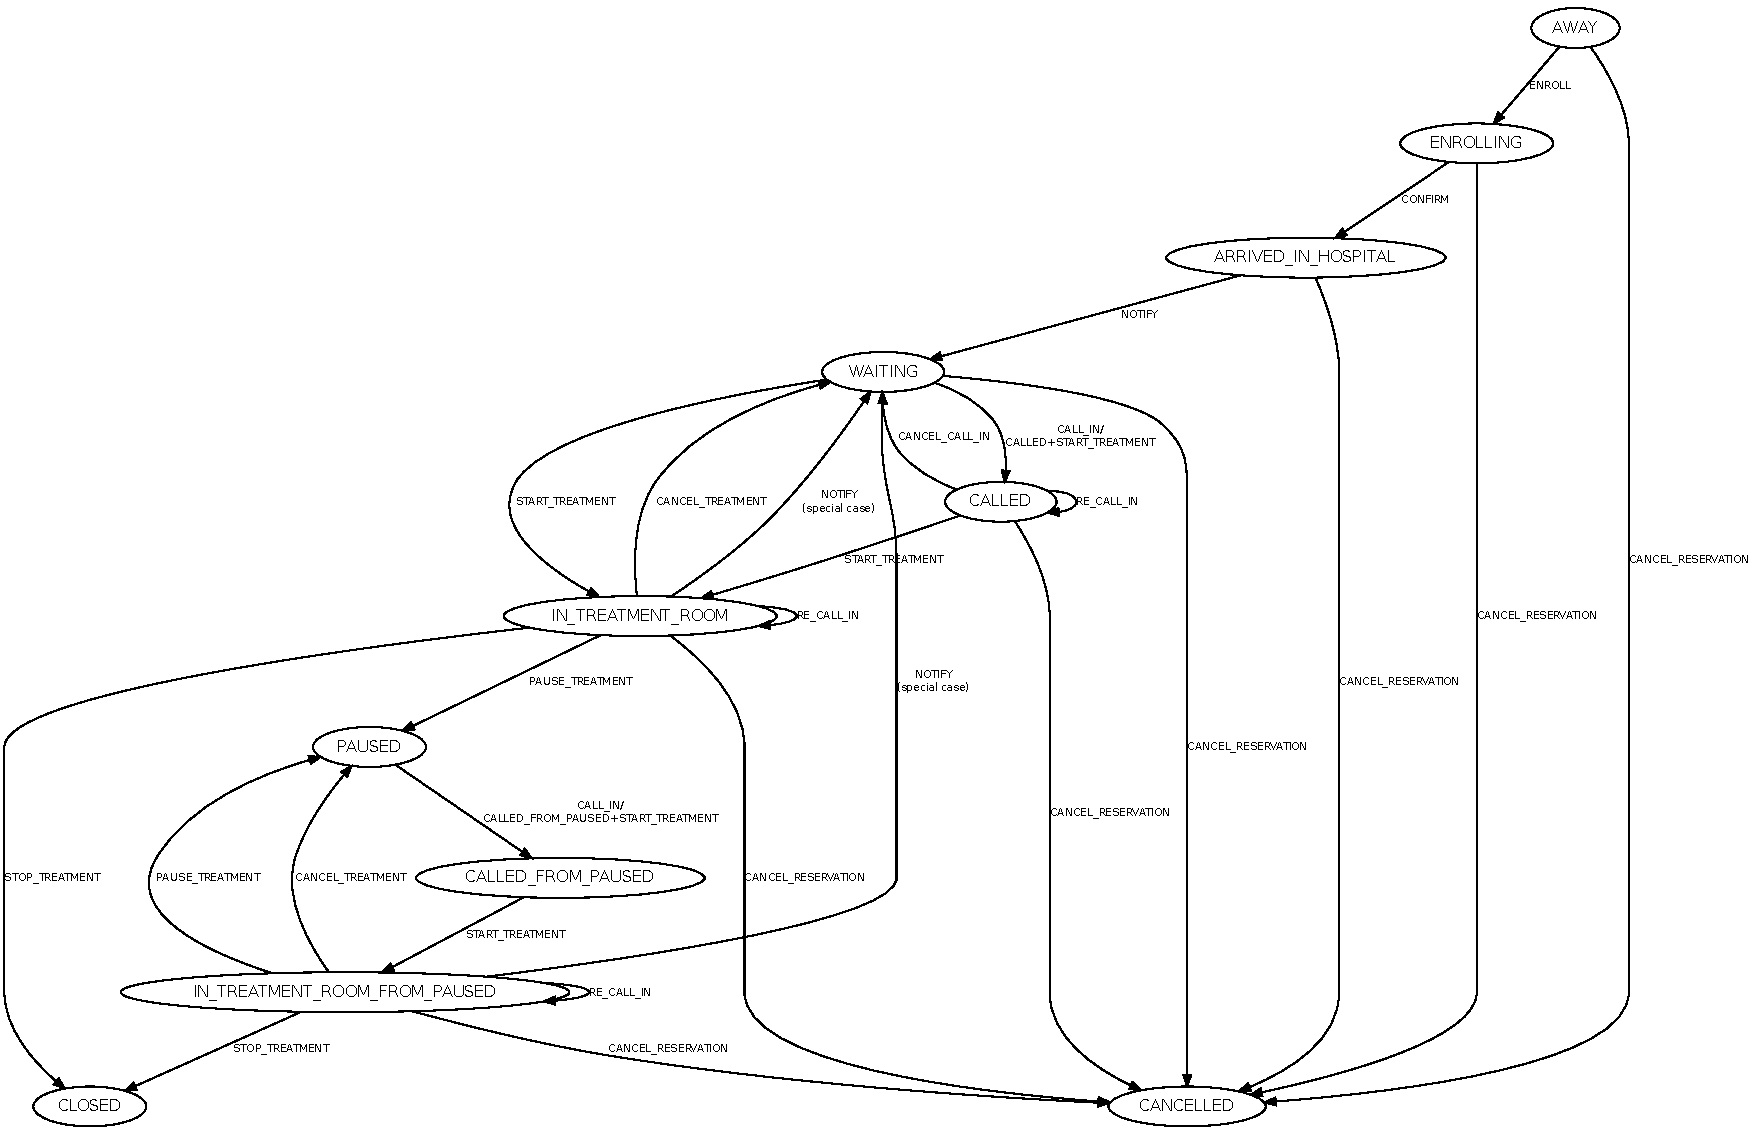
\includegraphics[width=0.8\textwidth]{images/patientFsm}
		\caption{State flow in X-Akseli system, version 1.18.3.}
		\label{fig:state}
	\end{center}
\end{sidewaysfigure}

One example visit is listed in Table~\ref{table:example}. Notice that, there are 6 events in this visit. However, the first two events \texttt{ENROLLING} and  \texttt{ARRIVED\_IN\_HOSPITAL} happened in less than 1 second. This also happens to the 4th and 5th events, \texttt{CALLED} and \texttt{IN\_TREATMENT\_ROOM}. It can be considered that the two events in these two pairs happen simutaneously. To reduce redundant information, in this thesis, only following 7 events are considered. They are: \texttt{ENROLLING}, \texttt{WAITING}, \texttt{IN\_TREATMENT\_ROOM}, \texttt{PAUSED}, \texttt{IN\_TREATMENT\_ROOM\_FROM\_PAUSED}, \texttt{CLOSED}, and \texttt{CANCELLED}.

\section{Problem Definition}
According to XXX, anomayly detection can be categorized into XXX types as follow:

The problem considered in this thesis can be classified as XXX.(Define what the feature of this type? why this type? why not other types? for example, extreme value detection.)

%The problem must have some background, otherwise it is not
%interesting.  You can explain the background here. Probably you should
%change the title to something that describes more the content of this
%chapter. Background consists of information that help other masters of
%the same degree program to understand the rest of the thesis.
%
%Transitions mentioned in Section~\ref{section:structure} are used also
%in the chapters and sections. For example, next in this chapter we
%tell how to use English language, how to find and refer to sources,
%and enlight different ways to include graphics in the thesis.
%
%\section{Language and Structure}
%
%Moreover, the transitions are also used in the paragraph and the
%sentence level meaning that all the text is linked together. For example,
%the word ``moreover'' here is one way, but of course you should use
%variation in the text. Examples of transitional devices (words) and
%their use can be found from writing guides, e.g. from the Online
%Writing Lab
%(OWL)\footnote{http://owl.english.purdue.edu/owl/resource/574/02/} of
%Purdue University or Strunk's Elements of
%Style\footnote{http://www.bartleby.com/141/}. Remember that footnotes
%are additional information, and they are seldom used.  If you refer to a source, you do no
%not use footnote. The right command for the references is \emph{cite}.
%
%The language used in the thesis should be technical (or
%scientifical). For example, the abreviations aren't used but all them
%are written open (i.e. ``are not''). Since the content itself is often
%hard to understand (and explain), the sentences should not be very
%long, use complex language with several examples embedded in the same
%sentence, and, also, seldom used words and weird euphemism or paraphrases
%can make the sentence hard to follow and to read it with only one
%time, and making everything even harder to understand all this without
%any punctuation marks makes the instructor cry and finally after
%trying to correct the language, you will get boomerang, and everyone's
%time has just been wasted.
%
%Please use proofreaders before sending even your unfinished version to
%the instructor and/or supervisor. You will get better comments when
%they do not need first proofread your text. Moreover, they can
%consentrate to the content better if the language and spelling
%mistakes are not distracting the reading. Several editors have their
%own proofreading tools, e.g. ispell in emacs. You can also use
%Microsoft Word to proofread your thesis: it can correct also some
%grammatical errors and not just misspelled words.
%
%Note also that if you have a section or a subsection, you have to have
%at least two of them, or otherwise the section or subsection title is
%unnecessary. Same with the paragraphs an: you should not have sections
%with only one paragraphe, and single sentence paragraph. Furthermore,
%always write some text after the title before the next level title.
%
%\section{Finding and referring to sources}
%
%Never ever copy anything into your theses from somebody else's text
%(nor your own previously published text). Never. Not even for starting
%point to be rewritten later. The risk is that you forgot the copied
%text to your thesis and end up to be accused of plagiarism. Plagiarism
%is a serious crime in studies and science and can ruin your career
%even its beginning. To repeate: never cut and paste text into your
%thesis!
%
%\subsection{Finding sources}
%
%All work is based on someone else's work. You should find the relevant
%sources of your field and choose the best of them. Also, you should
%refer to the original source where a fact has been mentioned first
%time. Remember source evaluation (criticism) with all sources you
%find.
%
%Good starting points for finding references in computer science are:
%\begin{itemize}
%% You can use this command to set the items in the list closer to each other
%% (ITEM SEParation, the vertical space between the list items)
%\setlength{\itemsep}{0pt}
%\item Nelli Portal (Aalto Library): \url{http://www.nelliportaali.fi}
%\item ACM Digital library: \url{http://portal.acm.org/}
%\item IEEExplore: \url{http://ieeexplore.ieee.org}
%\item ScienceDirect: \url{http://www.sciencedirect.com/}
%\item \ldots although Google Scholar (\url{http://scholar.google.com/}) will
%find links to most of the articles from the abovementioned sources, if you
%search from within the university network
%\end{itemize}
%
%Some of the publishers do not offer all the text of the articles
%freely, but the library has agreed on the rights to use the whole
%text. Thus, you should sometimes use computers in the domain of the
%university in order to get the full text. Sometimes the Nelli Portal
%can also help getting the whole article instead of just the abstract.
%The library has also brief instrucions how to find
%information~\cite{howfindinfo}.
%
%Instead of normal Google, use Google Scholar
%(\url{http://scholar.google.fi/}). It finds academic publications whereas
%normal Google find too much commercial advertisements or otherwise
%biased information. Wikipedia articles should be referred to in the master
%thesis only very, very seldomly. You can use Wikipedia for understanding
%some basics and finding more sources, but often you cannot be sure if
%the article is correct and unbiased.
%
%One important part of the sources that you have found is the reference
%list. This way you can find the original sources that all the other
%research of the field refer. Often you can also find more information
%with the name of the researchers that are often referred in the
%articles.
%
%\subsection{Referring to sources}
%
%The main point in referring to sources is to separate your own
%thinking and text from that of others. Facts of the research area can
%be given without reference, but otherwise you should refer to
%sources. This means two things: marking the source in the text where
%it has been used, and listing the sources usually in the end of the
%thesis in a way that help the reader to find the original source.
%
%There are several bibliography styles, meaning how to form the
%bibliography in the end of the thesis. Aalto's library has good
%instructions for many styles~\cite{bibinstructions}. You should ask
%from your supervisor or instructors which style you should use. This
%thesis template uses the number style that is often used in software
%engineering. The other style also used in the CS field,
%e.g. usability, is the Harvard style where instead of numbers, the
%reference is marked into the text with author's name and publishing
%year. Other areas use also many other styles for making the lists and
%marking the references.
%
%In addition to the list in the end of the thesis, you have to mark the
%source in the text where the source is used. There are three places
%for the reference: in a sentence before the period, in the end of a
%sentence after the period, or in the end of a paragraph. All of them
%have different meaning. The main point is that first you paraphrase
%the source using your own words and then mark the source. Next, we
%give short examples that are marked with \emph{emphasised text}.
%
%\emph{Haapasalo~\cite{HaapasaloThesis} researched database algorithms
%  that allows use of previous versions of the content stored in the
%  database.} This kind of marking means that this paragraph (or until
%the next reference is given) is based on the source mentioned in the
%beginning.  Giving the source you should use only the family name of
%the first author of the article, and not give any hints about what is
%the type of the article that is referred.
%
%\emph{B+-trees offers one way to index data that is stored in to a
%  database. Multiversion B+-trees (MVBT) offer also a way to restore
%  the data from previous versions of the database. Concurrent MVBT
%  allows many simultaneous updates to the database that is was not
%  possible with MVBT.~\cite{HaapasaloThesis}} When the marking is
%after the period, the reference is retrospective: all the paragraph
%(or after previous reference marking) is based on the source given in
%its end. If the content is very broad, you can start with saying
%\emph{According to Haapasalo}, then continue referring the source with
%several separate sentences, and in the end put the marking of your
%source \emph{ that shows that CMVBT are the
%  best. ~\cite{HaapasaloThesis}}.
%
%If your paragraph has several sources, the above mentioned styles are
%not proper. The reader of your thesis cannot know which of your
%sources give which of the statements. In this case, it is better to
%use more finegraded refering where the reference markings that are
%embedded in the sentences. For example, \emph{the multiversion B+-tree
%  (MVBT) index of Becker et al.~\cite{becker:1996:mvbt} allows database
%  users to query old versions of the database, but the index is not
%  transactional.
%  It's successor, the transactional MBVT (TMVBT), allows a single transaction
%  running in its own thread or process to update the database concurrently
%  with other transactions that only read the
%  database~\cite{haapasalo:2009:tmvbt}.
%  Further development, titled the concurrent MBVT (CMVBT),
%  allows several transactions to perform updates to the database at the same
%  time~\cite{HaapasaloThesis}}.
%  Here, the references are marked before
%  the period in the sentences where they are used.
%
%Finally, direct quotes are allowed. However, often you should avoid
%them since they do not usually fit in to your text very well. Using
%direct quotes has two tricks: quotation marks and the source.  \emph{
%  ``Even though deletions in a multiversion index must not physically
%  delete the history of the data items, queries and range scans can
%  become more efficient, if the leaf pages of the index structure are
%  merged to retain optimality.''~\cite{HaapasaloThesis}} Quotes are
%hard to make neatly since you should use only as much as needed
%without changing the text. Moreover, you often do not really
%understand what the author has mentioned with his wordings if you
%cannot write the same with your own words. Remember also that never
%cut and paste anything without marking the quotation marks right away,
%and in general, never cut and paste anything at all!
%
%Sometimes getting the original source can be almost impossible. In an
%extremely desperate situation, you can refer with structure \emph{mr
%  X~[\ldots] according to ms Y~[\ldots] defined that}, if you find a
%source that refers to the original source. Note also that the
%reference marking is never used as sentence element (example of how
%\textbf{not} to do it: \emph{\cite{HaapasaloThesis} describes
%an optimal algorithm for indexing multiversiond databases.}).
